\documentclass{beamer}

\usetheme{metropolis}
\definecolor{mediumred}{RGB}{180, 10, 5}
\setbeamercolor{frametitle}{bg=mediumred, fg=white}

\usepackage{tkz-graph}
\usepackage{tikz}
\usetikzlibrary{arrows,matrix,decorations.pathreplacing,positioning,chains,fit,shapes,calc} %
\usetikzlibrary{calc,patterns,decorations.pathmorphing,decorations.markings}

\usepackage{siunitx}
\usepackage{minted}

\usepackage{../../latex/custom}

\newcommand{\expe}[2]{\la #1, #2 \ra}

\newcommand\Wider[2][3em]{%
\makebox[\linewidth][c]{%
  \begin{minipage}{\dimexpr\textwidth+#1\relax}
  \raggedright#2
  \end{minipage}%
  }%
}

\title{Set Programming with JuMP}
\date{}
\author{Beno\^it Legat${}^*$, \emph{In collaboration with}: Rapha\"el M. Jungers${}^*$, Pablo A. Parrilo${}^\dagger$ and Paulo Tabuada${}^\ddagger$}
\institute{${}^*$ UCLouvain, ${}^\dagger$ MIT, ${}^\ddagger$ UCLA}

\makeatletter
\let\@@magyar@captionfix\relax
\makeatother

\begin{document}
\maketitle

  \begin{frame}
    \frametitle{Set program}
    \begin{block}{Set inclusion}
      Consider two sets $S \subseteq \R^n, T \subseteq \R^m$, matrices
      $A \in \R^{r \times n}, B \in \R^{r \times m}$:
      \[ A S \subseteq B T. \]
    \end{block}
    \begin{block}{Set program}
    Given fixed sets $T_i$, find sets $S_i$:
    \begin{align*}
      \max_{S_i, x_i} \quad & f(\vol(S_1), \ldots, \vol(S_n))\\
      A_j S_{a_j} & \subseteq B_j S_{b_j}\\
      S_i & \subseteq T_i\\
      x_{c_j} & \in S_{d_j}
    \end{align*}
    \end{block}
  \end{frame}

\begin{frame}{Stability of Hybrid Systems}
  \begin{center}
    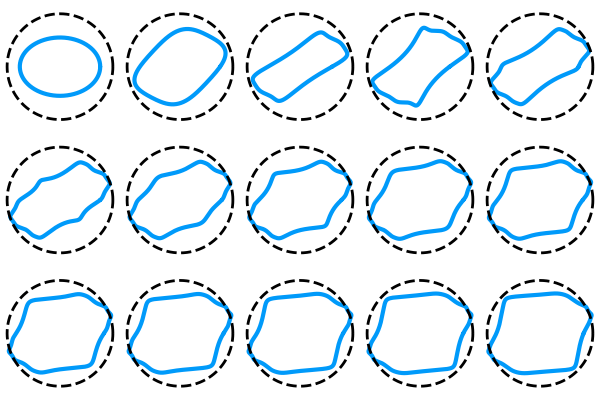
\includegraphics[width=0.8\textwidth]{../../latex/images/FinConjCounterEx.png}
  \end{center}

  \alert{Instability} may be certified using a \alert{low-rank} infeasibility certificate.

  See presentation at \emph{19th ACM International Conference on Hybrid Systems: Computation and Control,} (HSCC), 2016.
\end{frame}

\begin{frame}{Information Theory}
  \includegraphics[width=0.33\textwidth]{tetra0pm.png}~%
  \includegraphics[width=0.33\textwidth]{tetra0zy.png}~%
  \includegraphics[trim=6cm 2cm 6cm 7cm,clip,width=0.33\textheight]{tetra0bound15789.png}

  See presentation at \emph{37rd Symposium on Information Theory in the Benelux}, 2016.
\end{frame}

\begin{frame}{Safe Model Predictive Control}
  \begin{center}
    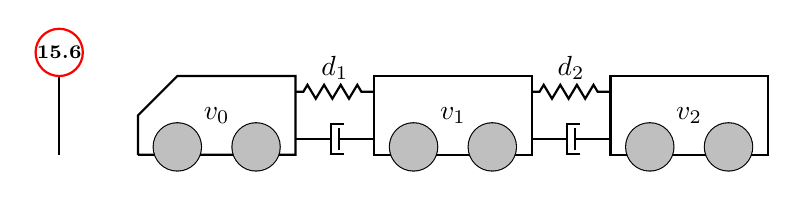
\begin{tikzpicture}
      \tikzstyle{spring}=[thick,decorate,decoration={zigzag,pre length=0.1cm,post length=0.1cm,segment length=6}]
\tikzstyle{damper}=[thick,decoration={markings,
  mark connection node=dmp,
  mark=at position 0.5 with
  {
    \node (dmp) [thick,inner sep=0pt,transform shape,rotate=-90,minimum width=10pt,minimum height=2pt,draw=none] {};
    \draw [thick] ($(dmp.north east)+(2pt,0)$) -- (dmp.south east) -- (dmp.south west) -- ($(dmp.north west)+(2pt,0)$);
    \draw [thick] ($(dmp.north)+(0,-4pt)$) -- ($(dmp.north)+(0,4pt)$);
  }
}, decorate]
\draw[thick] (0, 0) -- (2, 0) -- (2, 1) -- (0.5, 1) -- (0, 0.5) -- (0, 0);
\draw [spring] (2, 0.8) -- (3, 0.8);
\draw [damper] (2, 0.2) -- (3, 0.2);
\draw[thick] (3, 0) rectangle (5, 1);
\draw [spring] (5, 0.8) -- (6, 0.8);
\draw [damper] (5, 0.2) -- (6, 0.2);
\draw[thick] (6, 0) rectangle (8, 1);
\draw[thick] (0.5, 0.1) circle (0.3);
\fill[color=lightgray] (0.5, 0.1) circle (0.3);
\draw[thick] (1.5, 0.1) circle (0.3);
\fill[color=lightgray] (1.5, 0.1) circle (0.3);
\draw[thick] (3.5, 0.1) circle (0.3);
\fill[color=lightgray] (3.5, 0.1) circle (0.3);
\draw[thick] (4.5, 0.1) circle (0.3);
\fill[color=lightgray] (4.5, 0.1) circle (0.3);
\draw[thick] (6.5, 0.1) circle (0.3);
\fill[color=lightgray] (6.5, 0.1) circle (0.3);
\draw[thick] (7.5, 0.1) circle (0.3);
\fill[color=lightgray] (7.5, 0.1) circle (0.3);
\node at (1, 0.5) {$v_0$};
\node at (4, 0.5) {$v_1$};
\node at (7, 0.5) {$v_2$};
\node at (2.5, 1.1) {$d_1$};
\node at (5.5, 1.1) {$d_2$};

      \draw[thick] (-1, 0) to (-1, 1);
      \draw[thick,color=red] (-1, 1.3) circle (0.3);
      \node at (-1, 1.3) {\scriptsize \bf 15.6};
    \end{tikzpicture}

    \includegraphics[width=0.45\textwidth]{CruiseControlSets_d_u.png}
    ~
    \includegraphics[width=0.45\textwidth]{CruiseControlSets_v0_u.png}
  \end{center}

  See presentation at \emph{IFAC Conference on Analysis and Design of Hybrid Systems} (ADHS), 2018.
\end{frame}

\begin{frame}{Safe Stochastic Programming}
  \begin{center}
    \includegraphics[width=0.4\textwidth]{reservoir.jpg}~%
    \includegraphics[trim=.2cm .2cm .2cm .2cm, clip, width=0.6\textwidth]{ReservoirEllipsoidal.pdf}
  \end{center}
  See presentation at \emph{23rd International Symposium on Mathematical Programming} (ISMP), 2018.
\end{frame}

\begin{frame}[fragile]
  \frametitle{Example with ellipsoids: Model}
  Maximal volume ellipsoid (determinant):
  \begin{center}
    \includegraphics[width=\textwidth]{SetProg_Ellipsoid_AE.png}
  \end{center}
  Maximal sum of the squares of the semi-axes of the ellipsoid (trace):
  \begin{minted}{julia}
@objective(model, Max,
           L1_heuristic(volume(S), [1.0, 1.0]))
  \end{minted}
\end{frame}

\begin{frame}{Example with ellipsoids: Primal Solution}
  \begin{center}
    \includegraphics[width=\textwidth]{SimpleControlledInvariantEllipsoid.png}~%
  \end{center}
\end{frame}
\begin{frame}{Example with ellipsoids: Polar Solution}
  \begin{center}
    \includegraphics[width=\textwidth]{SimpleControlledInvariantPolarEllipsoid.png}
  \end{center}
\end{frame}

\begin{frame}[fragile]
  \frametitle{Example with polynomial sublevel set: Model}
  \begin{minted}{julia}
@variable(model, S, PolySet(degree=d, convex=true,
                            symmetric=true))
  \end{minted}
  Use L1 norm as volume heuristic.
\end{frame}

\begin{frame}{Example with polynomial sublevel set: Primal Solution}
  \begin{center}
    \includegraphics[width=\textwidth]{SimpleControlledInvariantPolySet.png}
  \end{center}
\end{frame}
\begin{frame}{Example with polynomial sublevel set: Polar Solution}
  \begin{center}
    \includegraphics[width=\textwidth]{SimpleControlledInvariantPolarPolySet.png}~%
  \end{center}
\end{frame}

\begin{frame}[fragile]
  \frametitle{Set variables}
  \begin{minted}{julia}
function JuMP.build_variable(
    _error, info::JuMP.VariableInfo, set::AbstractSetVariable)
    if info.has_lb || info.has_ub || info.has_fix ||
       info.binary || info.integer || info.has_start
        _error(...)
    end
    return set
end
function JuMP.add_variable(
    model::JuMP.AbstractModel, set::AbstractSetVariable,
    name::String)
    vref = SetVariableRef(...)
    push!(data(model).variables, vref)
    return vref
end
  \end{minted}
\end{frame}

\begin{frame}
  \frametitle{Parsing set constraints}
  \begin{center}
    \includegraphics[width=\textwidth]{SetProg_parse_constraint.png}
  \end{center}
\end{frame}

\begin{frame}[fragile]
  \frametitle{Store set constraints}
  \begin{minted}{julia}
function JuMP.build_constraint(
    _error::Function, subset, sup_powerset::PowerSet;
    kws...)
    InclusionConstraint(subset, sup_powerset.set, kws)
end
function JuMP.add_constraint(
    model::JuMP.Model, constraint::SetConstraint,
    name::String="")
    d = data(model)
    index = ConstraintIndex(d.last_index += 1)
    d.constraints[index] = constraint
    d.names[index] = name
    return JuMP.ConstraintRef(model, index, SetShape())
end
  \end{minted}
\end{frame}

\begin{frame}[fragile]
  \frametitle{Optimize hook}
  \verb|create_spaces|: Find dimensions and
  representation (e.g. polar/dual or not)
  \begin{minted}{julia}
function optimize_hook(model::JuMP.AbstractModel)
    d = data(model)
    clear_spaces(d)
    create_spaces(d)
    load(model, d)
    JuMP.optimize!(model, ignore_optimize_hook = true)
end
  \end{minted}
\end{frame}

\begin{frame}[fragile]
  \frametitle{Load set constraints}
  S-procedure:
  \begin{align*}
    Q & \subseteq P\\
    x^\top Qx \le 1 & \Rightarrow x^\top Px \le 1\\
    x^\top Px & \le x^\top Qx \quad \forall x\\
    Q - P & \text{ is PSD}
  \end{align*}
  \begin{minted}{julia}
function JuMP.build_constraint(
    _error::Function, subset::Ellipsoid,
    sup_powerset::PowerSet{<:Ellipsoid})
    Q = subset.Q
    P = sup_powerset.set.Q
    JuMP.build_constraint(_error, Symmetric(Q - P),
                          PSDCone())
end
  \end{minted}
\end{frame}

\begin{frame}[fragile]
  \frametitle{Polar inclusion}
  \begin{minted}{julia}
function JuMP.build_constraint(
    _error::Function, subset::Sets.Polar,
    sup_powerset::PowerSet{<:Sets.Polar})
    S = subset
    T = sup_powerset.set
    JuMP.build_constraint(
        _error, Sets.polar(T), PowerSet(Sets.polar(S)))
end
  \end{minted}
  \begin{minted}{julia}
function JuMP.build_constraint(
    _error::Function, subset::Sets.Polar,
    sup_powerset::PowerSet{<:Polyhedra.HalfSpace})
    point = sup_powerset.set.a / sup_powerset.set.b
    JuMP.build_constraint(_error, point, Sets.polar(subset))
end
  \end{minted}
\end{frame}

\begin{frame}[fragile]
  \frametitle{Future work}
  \begin{itemize}
    \item Rely on \verb|MathematicalSets| to represent sets.
    \item Polyhedra solver (CDD, LazySets, ...)
    \item Direction objective: Ellipsoid (SDP), polynomial (SOS), polyhedra (SDDP).
  \end{itemize}
\end{frame}

\end{document}
